\chapter{A stochastic agent-based network model}
\label{ch:abms}
\section{Agent-based models}
Agent-based modelling is a computational method that models interacting individuals in an environment using a `bottom-up' approach\cite{abm-gilbert}. The individuals are given preferences, actions available to them and ways to perceive not only themselves and their environment but also other agents. This method has proved useful in modelling a wide variety of complex systems in biology\cite{kroese-uppal}, social science\cite{epstein} and economics\cite{abm-economics}.\\
\\
Its utility derives from allowing researchers to solely define the characteristics of the individuals without saying anything explicit about the system they are trying to model. They then see what happens when those individuals are free to interact with each other and the environment in the ways defined. This lets researchers to model complex system-wide phenomena without making any system-wide assumptions.
\subsection{The components}
An agent-based model (ABM) has four essential elements: agents, the environment, the rules that define how the two of these work together and time.\\
\\
%agents
The agents can represent anything from an individual person to a company, from a bacteria to a country. Anything that has `agency' can be an agent in an ABM. That is, anything that has the ability to act. They are programmed to react to other agents, which may or may not be of the same type. So a person can interact with another person but could also interact with an agent that is a frog or a country.\\
\\
%Environment
The environment is a virtual world the agents both exist in and interact with\cite{abm-gilbert}. The environment may be abstract such as a network with the agents as nodes and an edge between two nodes signifying that those agents can interact with each other. However, it might also be very specific and concrete such as a geographically accurate rendering of a city.\\
\\
The rules bind these two elements. They define things like how many agents of each type there are in the environment, when agents can act and who with.\\
\\
%Time
For an ABM to be a useful model of a system by definition the agents need to act. For something to act, we need time to evolve. So time is an inherent part of ABMs. However, representing time in any computer program is a challenge. One can either approximate continuous time or be explicitly discrete. Due to the difficulties of approximating continuous time, most ABMs have time incrementing in discrete steps. We call the units of time \textit{ticks}.\\
\\
To make this a bit easy to grasp and see how it works in practice, we will look at one in-depth but simple example.

\subsection{Example: Boltzmann wealth model}\label{sec:boltzmann-wealth}
%\subsubsection{Introduction}
We will build a simple agent-based model to illustrate how they typically work. Taking a short break from the area of epidemiology and revolutions, we will try to model the unequal distribution of wealth in society. Econophysics is a trendy area of research, applying concepts from statistical mechanics to the study of economics\cite{econophysics2}. The model we will look at will be inspired by this area and, in particular, a model of Dr\u agulescu\cite{econophysics1} and Yakovenko\cite{boltzmann-tutorial}. The model is incredibly simple with only one type of agent, a minimal environment and just three rules. Despite its simplicity, this model can provide interesting and unexpected results.
\subsubsection{Setup}
%Agents, environment, time
In our model the agents are people. They have a non-negative integer amount of wealth $w\in\mathbb{N}^{\geq 0}$. They also have the ability to transfer money, if they have any, to other agents. The environment connects all agents to each other, allowing any agent to transfer money to any other. We will use discrete time in this model.\\
\\
%\paragraph{Rules}
The rules are simple:
\begin{enumerate}[
%	nosep,
%	label={Rule \arabic*}
	]
	\item\label{} There are $n$ agents.
	\item\label{} All agents start with $1$ unit of wealth.
	\item\label{} At each time-step, each agent that has at least one unit of wealth gives one unit to another agent, chosen randomly.
	\setcounter{rule}{\value{enumi}}
\end{enumerate}
\subsubsection{Implementation}
ABMs are essentially computer programs and so to implement the ideas above we need to write a program that will run in line with the set-up we have described.\\
\\
The implementation of an agent-based model typically has two main classes: the model and the agents. The model class defines the environment, the rules and controls time. It also holds the global variables such as the number of agents and is in charge of keeping track of all the agents. The agent class defines the interacting individuals. Typically this class will hold an agent's own properties and will define the functions that allow the agent to sense their environment and interact with other agents.\\
\\
%\paragraph{Implementing This}
The rules tell us what we need in the program.
\begin{enumerate}[
%	nosep,
%	label={From rule \arabic*}
	]
	\item\label{} We need the model class to hold an integer $n$, the number of agents in the model. We also need the model to have a way of creating agents.
	\item\label{} We need each agent class to hold the units of wealth that they have. We also need the model class to initialise each agent with $1$ unit of wealth.
	\item\label{} The agent class needs a function to distribute wealth. At each tick, if the agent has positive wealth, they decrease their wealth by 1 and increase the wealth of another agent by $1$.
\end{enumerate}
An example of a bare bones implementation of this is:
\lstinputlisting[language=python]{../Code/illustrative/boltzmann-wealth/bare-bones-1.py}
Note that we also assign each agent a `unique ID'. This is helpful for collecting data about the model, in particular for creating visual representations of the model or alternatively looking at typical behaviour of individual agents.
\subsubsection{Running the model}
We still need to add a few lines to make the code run and get a visual output. Letting it run for $100$ ticks with $100$ agents and plotting the results using
\lstinputlisting[language=python]{../Code/illustrative/boltzmann-wealth/bare-bones-2.py}
we get figure \ref{fig:single-init-1}.
\begin{figure}[h!]
	\centering
	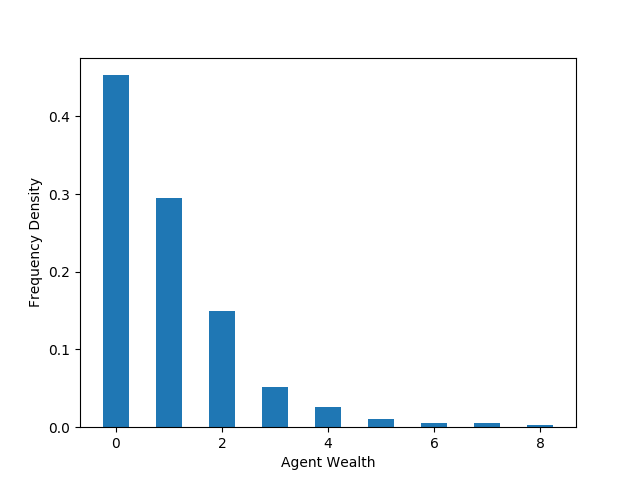
\includegraphics[width=.9\linewidth]{boltzmann-wealth/single-init-1.png}
	\caption{Graph of the density of agent's wealth after one $100$ step run of the Boltzmann wealth model with $100$ agents with initial wealth $1$}
	\label{fig:single-init-1}
\end{figure}
Though the program begins with the money equally spread throughout the population, it quickly becomes centred around a few very wealthy individuals. Around half of the population end up with nothing at all.\\
\\
%\paragraph{Batch Run}
The above graph was generated using just a single run of the program. One way we can get a clearer and firmer understanding of the system is to do `batch runs' where we run the simulation multiple times with the same parameters and compile all of the results. The following graph comes from running 100 of the simulations and creating a histogram of the wealth of the agents at the end.
\begin{figure}[!h]
	\centering
	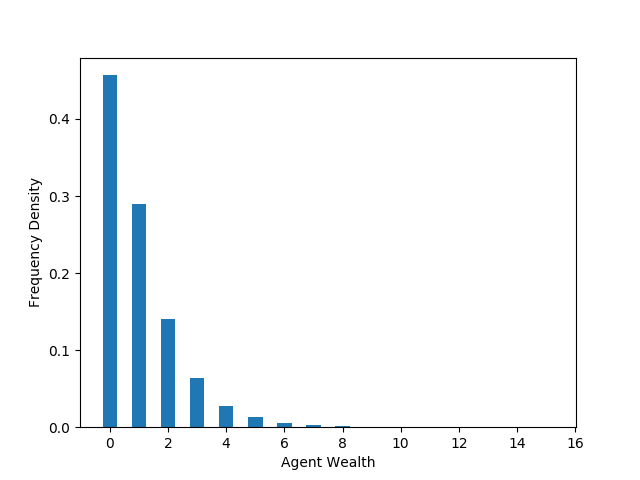
\includegraphics[width=.9\linewidth]{boltzmann-wealth/batch-init-1.png}
	\caption{Batch run of the Boltzmann Wealth model}
	\label{fig:batch-init-1}
\end{figure}
%would be cool to fit boltzmann curve to this
This shows the same disparity, perhaps even more starkly. Counter-intuitively, at least to me, despite having a constant process of redistributing wealth that seems to be in favour of the poor, we end up with a vastly unequal distribution. Almost half of all agents have 0 units of wealth while less than $10\%$ have $4$ or more. One agent in one of the runs ends with a wealth of $15$. Through a simple and easily comprehensible system we have found some intriguing results.\\
\\
One of the benefits of defining a social system as a program is that it makes it easy to run social experiments that would be difficult or unethical in real life. For example we can ask: what about if there is just more money around? Would that make the wealth distribution more equal? Exploring this is as easy as editing one initial value. If we start each individual with an initial wealth of $10$, though it takes longer to get there, we still end up with this inequality eventually. After 10000 ticks we end up with Figure \ref{fig:single-init-10}.
\begin{figure}[h!]
	\centering
	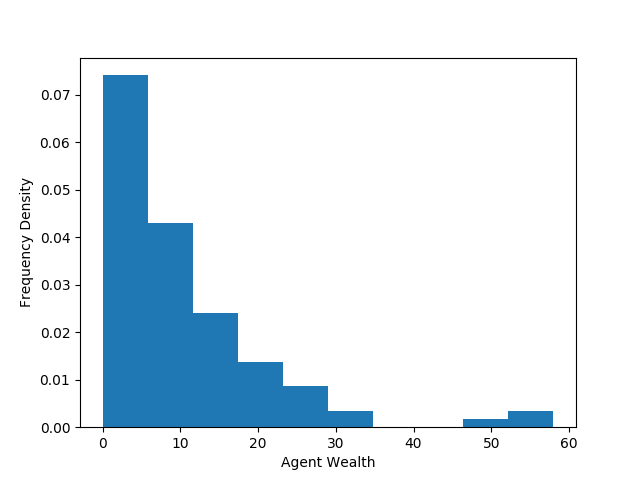
\includegraphics[width=.9\linewidth]{boltzmann-wealth/single-init-10.png}
	\caption{Histogram showing the result of increasing agent's initial wealth to $10$ on the Boltzmann wealth model.}
	\label{fig:single-init-10}
\end{figure}
So, in this system at least, economic inequality cannot be fixed by more money.\\
\\
We can then analyse this data as if it was field data. The fact that the distribution of wealth seems to move towards the same shape suggests some underlying equilibrium distribution. It turns out that the distribution of the wealth resulting from this model is actually a Boltzmann distribution\cite{dragulescu}. This is an exponential distribution typically linked to stochastic systems that try to reduce their energy potential.\\
\\
ABMs typically need some exterior reassurance that they are actually modelling the real world. Otherwise one can make many simplifications and assumptions and end up with a model that may or may not represent the system it is attempting to talk about. In this case one might consider real datasets of the income of a population. Indeed datasets show that income in the U.S.A. is distributed in a similar way to a Boltzmann distribution\cite{econophysics1}.\\
\\
If the data and model agree, researchers can use the model's results as evidence for bolder theses. In this case, researchers have argued that the Boltzmann distribution is in fact the \textit{expected} distribution of wealth in a capitalist society\cite{econophysics1}. The idea that this is a fundamental fact can be tested by seeing the result's robustness to different parameter values, rules and even different models. In this way, ABMs provide an interesting way to move back and forth between the world of theory and real world data.
\section{Social networks}
%\paragraph{Introduction}
In the Boltzmann wealth model the individuals exist in a very abstract space in which they interact with every other individual. In practice this is quite an unusual situation, as in general each person has some people they are more likely to interact with than others. People interact with the same people each day and have different relationships with others: friends, colleagues, stranger, daughter, spouse. This affects the interactions. This is also not unique to people. Companies, animals and countries have similar preferences and histories.\\
\\
We can consider each agent in a population as a node and we have an edge connecting two nodes if the two people have some form of social interaction such as friendship or acquaintance. This defines a social network\cite{networks}. An example of a social network is given by the author's Facebook friend network in Figure \ref{fig:facebook-network}.
\begin{figure}[h]
	\centering
	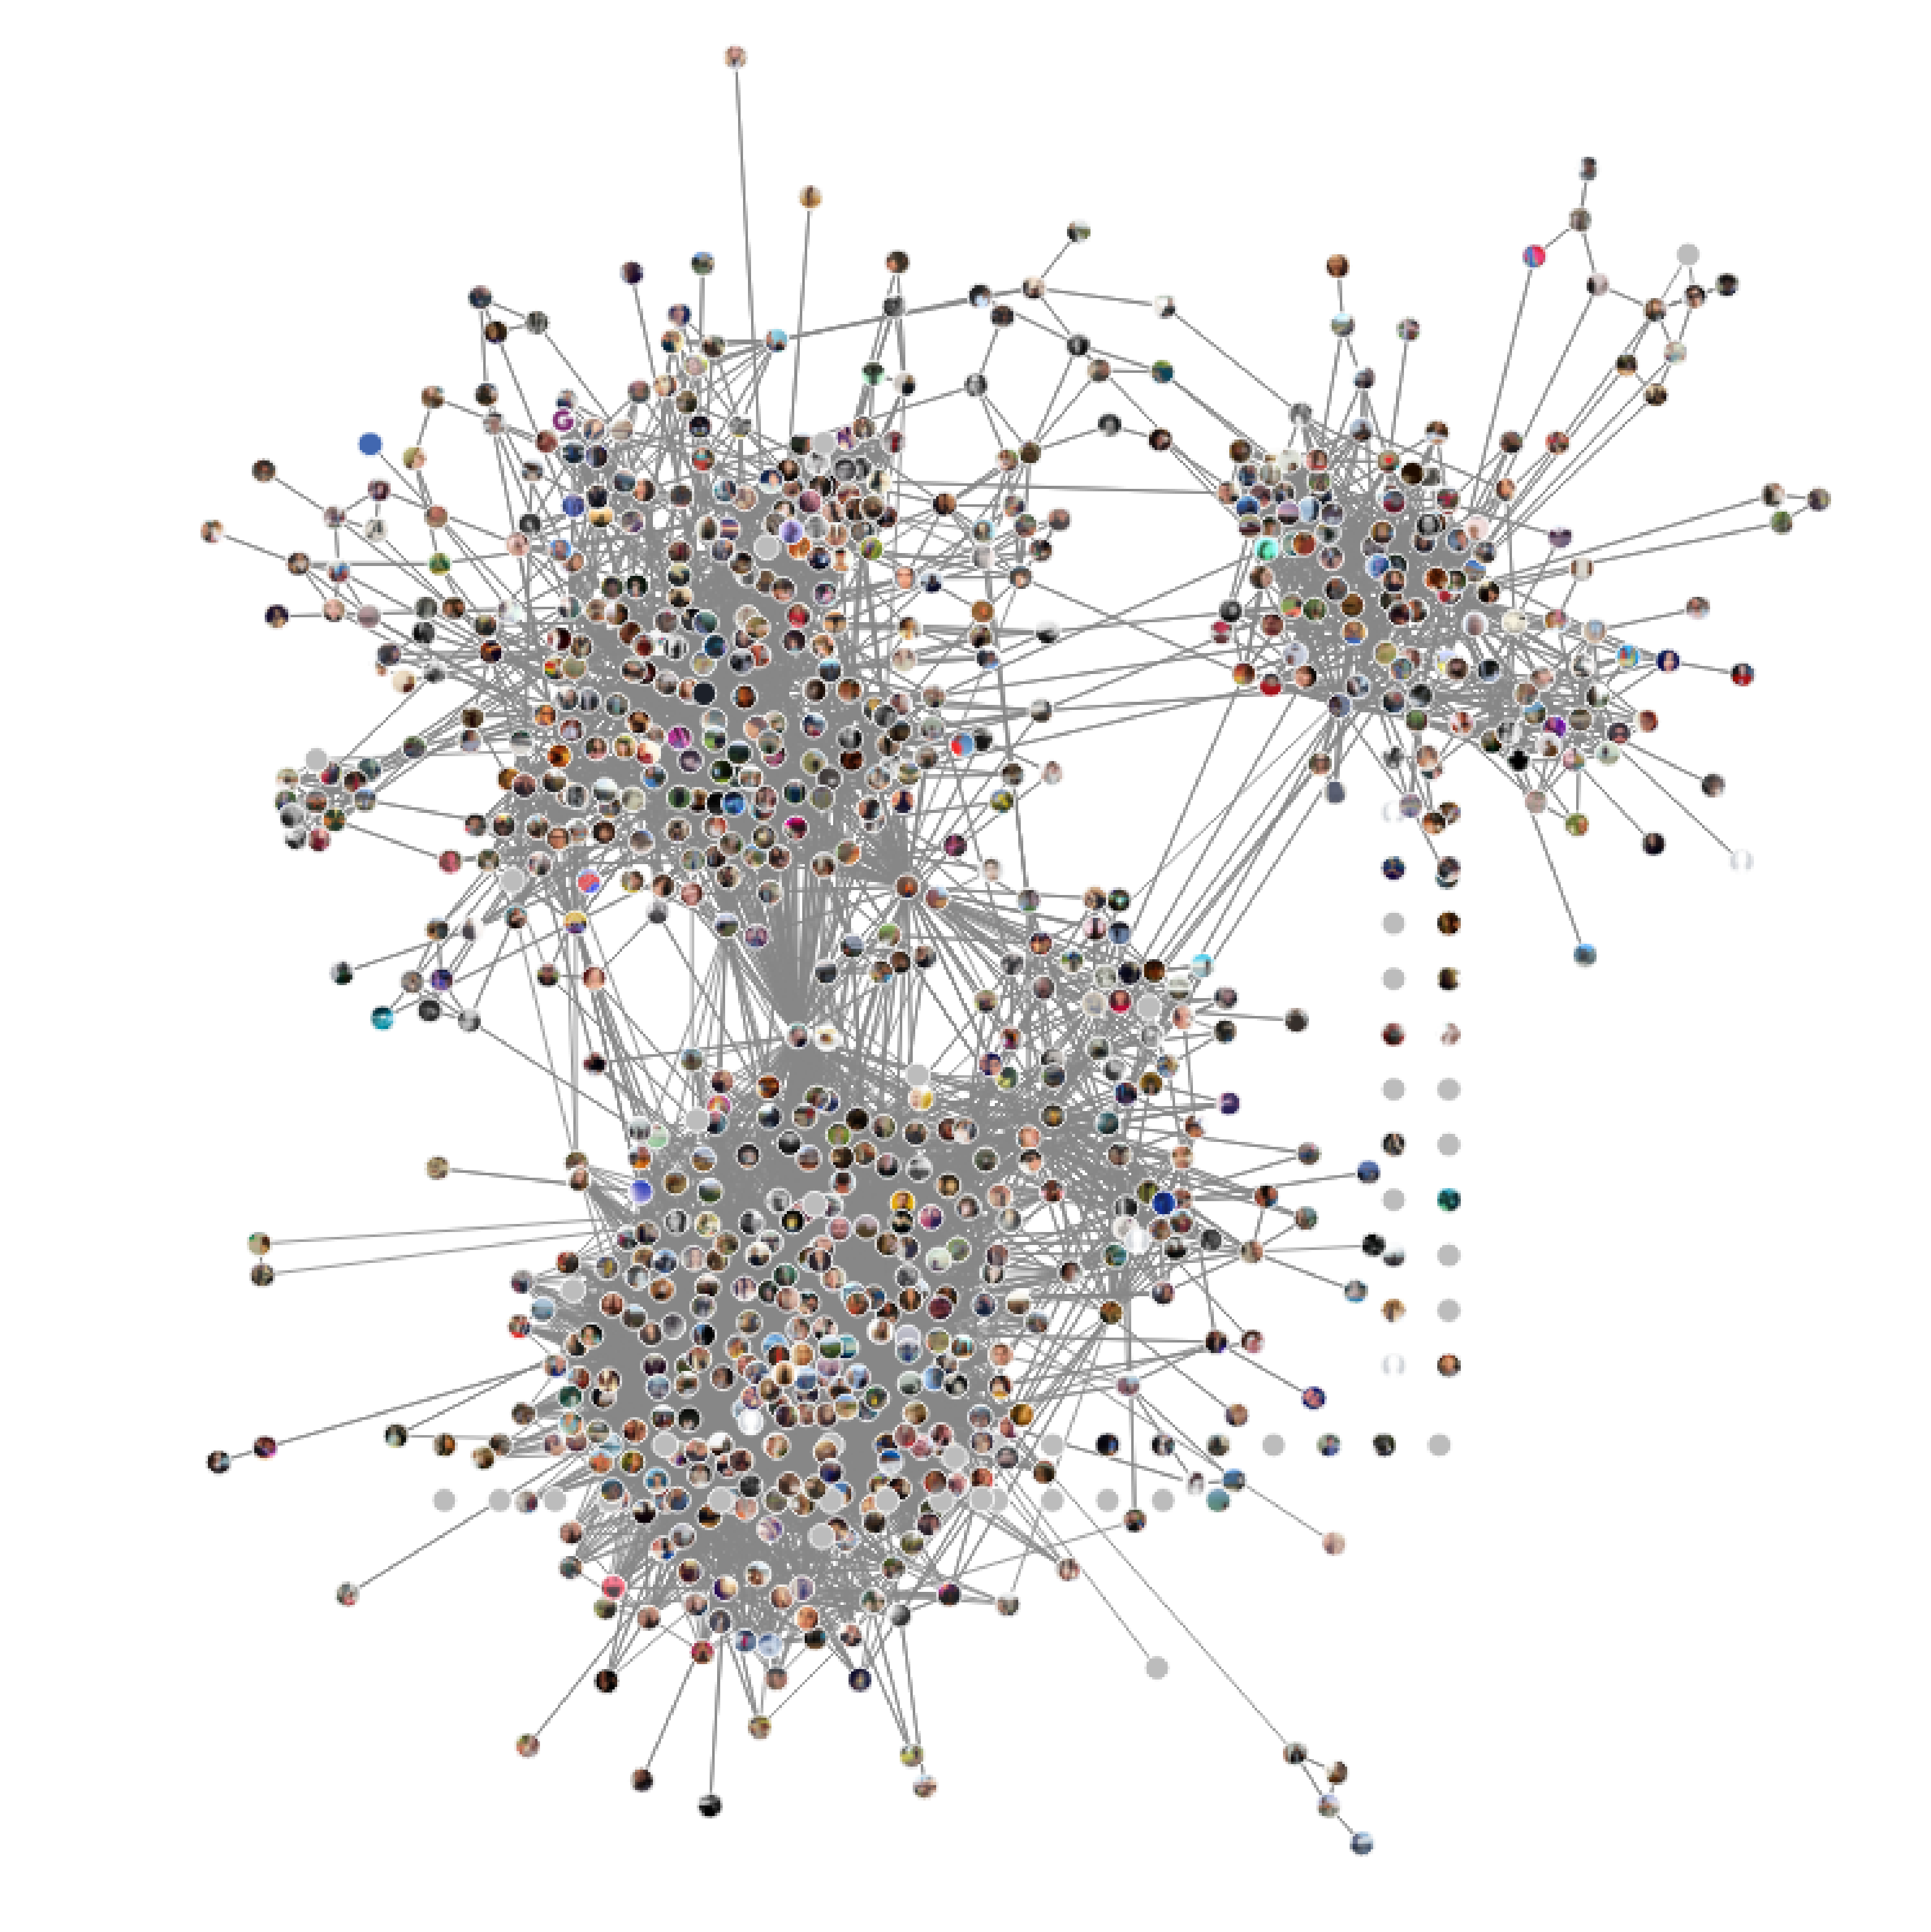
\includegraphics[width=.7\linewidth]{social-networks/joe-facebook-network-cropped}
	\caption{The author's Facebook friend network. Each node represents a Facebook friend and an edge between two nodes represents that those two people are friends on Facebook. Three main groups are revealed. The lower left contains people from Newcastle where I grew up. The top left are people from Manchester and university. The top right are people from Montreal where I studied for a year.}
	\label{fig:facebook-network}
\end{figure}\\
\\
For the success of an ABM that has a network structure underlying it, it is important to ensure that the network of the simulation accurately represents the features of a typical network. In particular for our case of modelling a revolution it is important to find a social network that accurately reflects the social graph of influence around transmitting political views and actions between citizens.\\
\\
There are two main ways we can find suitable networks to use in a model. Firstly, we can consider random graphs. These are a general species of graphs that are formed by a set of rules and reflect some aspect of real-life networks. The second option is to use datasets of real-life networks. Both have their merits and drawbacks.
\subsection{Random graphs}
%--Features of social networks: random, power-law tail, high clustering.--\\
A key feature of real-life networks is that they are irregular. They are much messier than well-ordered graphs such as complete graphs and lattices (see section \ref{sec:graph-theory}). To approximate this we need to look at graphs that can incorporate probability into some aspects of its structure. There are three main species of random graph we will look at: the Erd\H{o}s-R{\'e}nyi graph, scale-free graphs and small-world graphs.
%\\\\
%We also desire it to have a power-law tail and high clustering.
\subsubsection{Erd\H{o}s-R{\'e}nyi graph, $G(n,p)$}
The prototypical and perhaps simplest random graph is the Erd\H{o}s-R{\'e}nyi graph\footnote{Also known as the Poisson random graph, the Bernoulli random graph or simply the random graph.} $G(n,p)$. It is so prototypical it is often called \textit{the} random graph. It is defined in terms of two parameters: the number of nodes $n$ and the probability that there is an edge between any two nodes $p$. Figure \ref{fig:erdos-renyi-graphs} shows three graphs generated by this model.
\begin{figure}
	\centering
	\begin{subfigure}{.45\textwidth}
		\centering
		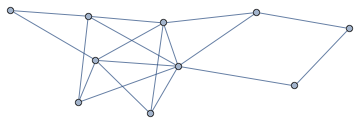
\includegraphics[width=1\linewidth]{erdos-renyi/G(10,0'5).png}
		\caption{$G(10,0.5)$}
		\label{fig:K5}
	\end{subfigure}
\begin{subfigure}{0.5\textwidth}
	\centering
	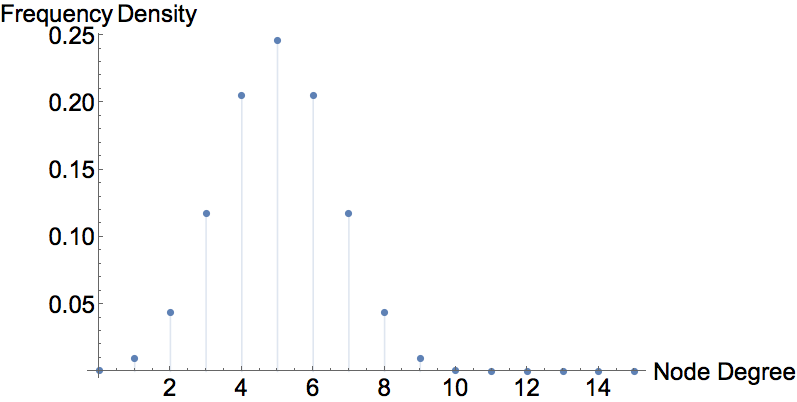
\includegraphics[width=1\linewidth]{erdos-renyi/e-r-prob-dist-1.png}
	\caption{$G(10,0.5)$}
	\label{fig:K5}
\end{subfigure}
	\begin{subfigure}{.45\textwidth}
		\centering
		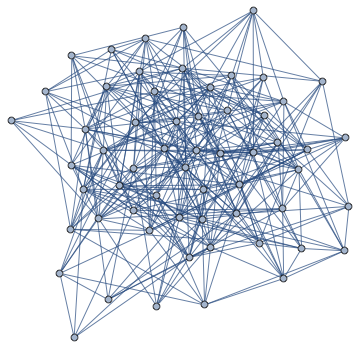
\includegraphics[width=1\linewidth]{erdos-renyi/G(59,0'2).png}
		\caption{$G(59,0.2)$}
		\label{fig:K16}
	\end{subfigure}
\begin{subfigure}{0.5\textwidth}
	\centering
	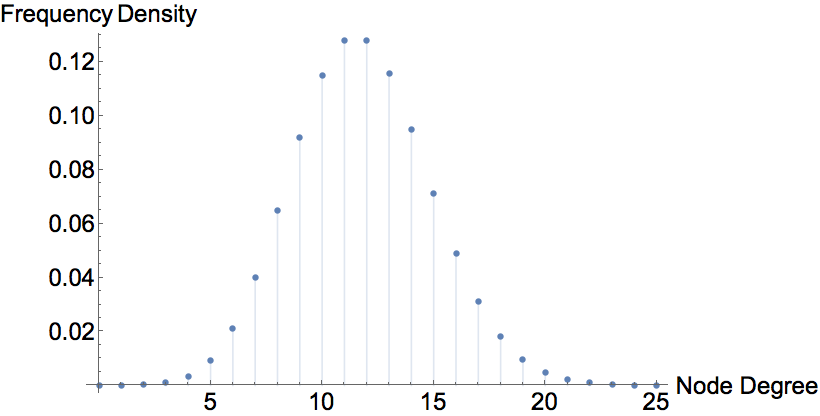
\includegraphics[width=1\linewidth]{erdos-renyi/e-r-prob-dist-2.png}
	\caption{$G(10,0.5)$}
	\label{fig:K5}
\end{subfigure}
	\begin{subfigure}{.45\textwidth}
		\centering
		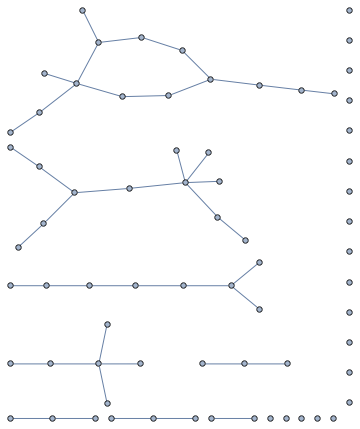
\includegraphics[width=1\linewidth]{erdos-renyi/G(70,0'02).png}
		\caption{$G(70,0.02)$}
		\label{fig:K16}
	\end{subfigure}
\begin{subfigure}{.5\textwidth}
	\centering
	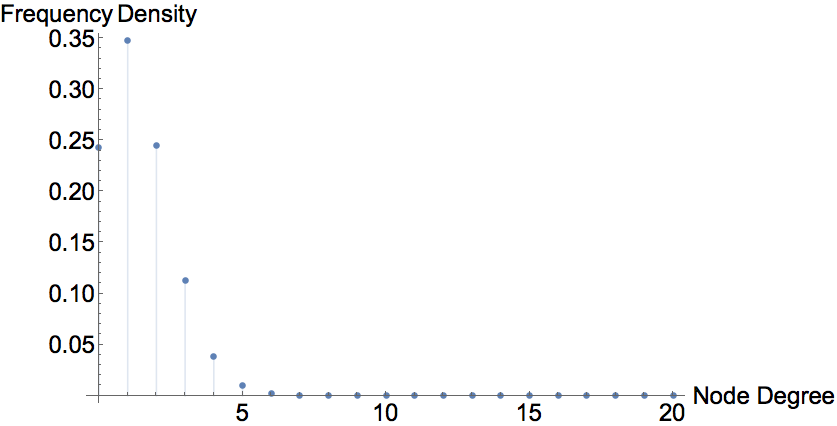
\includegraphics[width=1\linewidth]{erdos-renyi/e-r-prob-dist-3.png}
	\caption{$G(70,0.02)$}
	\label{fig:K16}
\end{subfigure}
	\caption{Examples of Erd\H{o}s-R{\'e}nyi graphs on the left with the expected probability distributions of Erd\H{o}s-R{\'e}nyi graphs with these parameters.}
	\label{fig:erdos-renyi-graphs}
\end{figure}
%\paragraph{Limitations}
Unfortunately $G(n,p)$ has two major limitations in modelling real-world social networks: it has an unrealistic degree distribution and it has low clustering.\\
\\
%\paragraph{Degree Distribution}
Firstly, the degree distribution of $G(n,p)$ is a binomial distribution. That is to say the probability of a node being connected to $k$ others is:
\begin{equation}
	p_k=\binom{n-1}{k}p^k(1-p)^{n-1-k}
\end{equation}
This is easily understood. Each node can be connected to $n-1$ others, there are $\binom{n-1}{k}$ ways to be connected to $k$ of them, and the probability of having exactly $k$ edges is $p^k(1-p)^{n-1-k}$. This means that the degree of the vertices has the binomial distribution $B(n-1,p)$. However, the binomial distribution does not have `heavy tails', a feature often found in real-world networks including social networks\cite{barabasi-albert}. This limits the ability of $G(n,p)$ to model social networks.\\
\\
It is worth explaining the meaning of `heavy-tailed'. Qualitatively this means that in a sample from a heavy-tailed distribution you are more likely to get a small number of very high values. Quantitatively it means that the right tail of the distribution has a heavier tail than the exponential distribution\cite{heavy-tailed}. That means that the probability distribution function has higher values for large $x$ (Figure \ref{fig:heavy-tailed}).
\begin{figure}
	\centering
	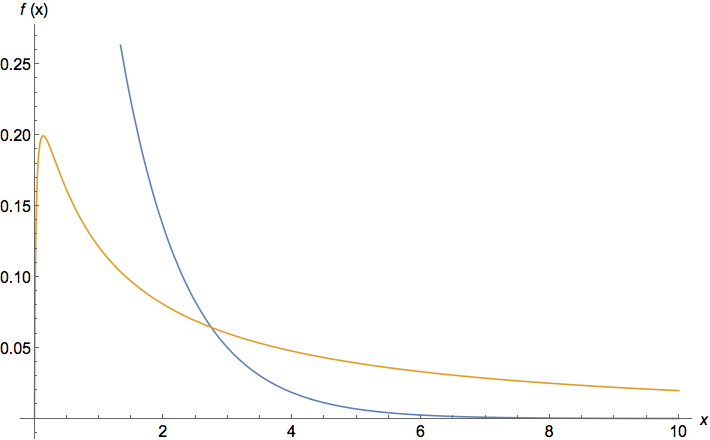
\includegraphics[width=.9\linewidth]{erdos-renyi/heavy-tailed.png}
	\caption{A graph showing the pdf of the exponential distribution in blue against the `heavy-tailed' log-normal distribution in orange.}
	\label{fig:heavy-tailed}
\end{figure}
%\textit{Mark: say something about what it means to be heavy-tailed}
\label{mmd}
\\
\\
%\paragraph{Clustering}
Secondly, $G(n,p)$ does not show nodes clustering as much as a real-world network. The clustering coefficient, $C$ is a measure of how likely nodes are to be in clusters. Formally, it is the probability that two neighbours of a vertex are also neighbours of each other\cite{networks}. In the Erd\H{o}s-R{\'e}nyi graph, this probability is independent of all other edges. Hence the expectation of the clustering coefficient is simply $\langle C\rangle=p$.\\
\\
This says that two neighbours are just as likely to be connected if they have a neighbour in common as if they do not. Most real social networks have high clustering, resulting from a phenomena called triadic closure\cite{simmel}\cite{strength-weak}. This just means that two of your friends are more likely to know each other than two random people. To see this, think of all your mutual friends and also how you tend to meet your friend's friends eventually.\\
\\
%\subsubsection{Summary}
Whilst the Erd\H{o}s-R{\'e}nyi graph does not provide an accurate representation of most social networks, its simplicity makes it useful for running some models. However, we will also consider some graphs that avoid the problems faced by the Erd\H{o}s-R{\'e}nyi graph.
\subsubsection{Scale-free graphs: the Barab\'asi-Albert model}
Scale-free graphs are defined as graphs that have distributions of node degree that follow a power law. That is the probability of a node being connected to exactly $k$ others is $p_k\sim k^{-\gamma}$ where $\gamma>0$. Early promoters of scale-free networks claim that they are prevalent throughout real-world networks\cite{barabasi-albert}. However, recent reviews of large datasets suggest that there is limited evidence for this\cite{scale-free-rare}.\\
%\\
%\textit{Say what scale-free means here}
\label{mmd}
%\\
\\
Regardless, the Barab\'asi-Albert model is one of the most widely known models that can generate scale-free networks. It does so by generating graphs by a process of \textit{preferential attachment}\cite{barabasi-albert}. 
\begin{figure}
	\centering
	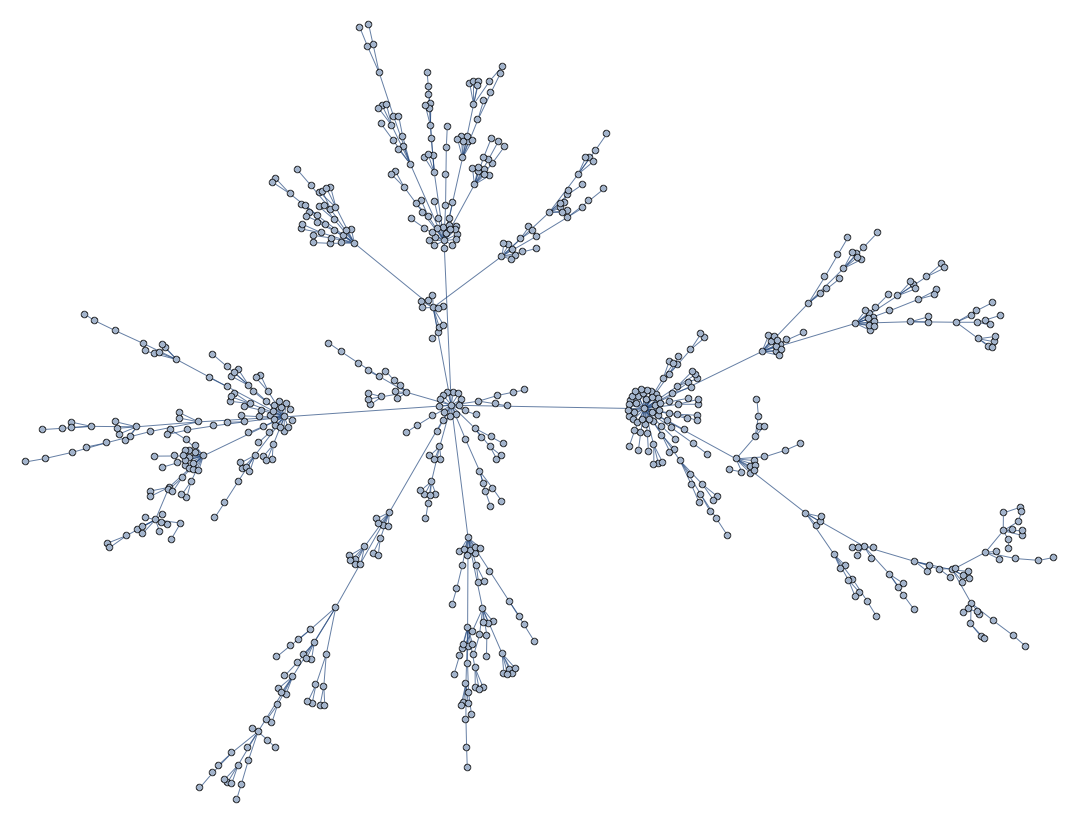
\includegraphics[width=.9\linewidth]{barabasi-albert/700.png}
	\caption{A graph with 700 nodes created from the Barab\'asi-Albert model}
	\label{fig:ba-700}
\end{figure}
%\paragraph{Setup}
A Barab\'asi-Albert graph is made by the following process. Start with a graph of two connected nodes. We take discrete steps in time and at each step we add one node and connect it to one existing node. The existing node is chosen with probability proportional to its degree. That is, a node with degree $k$ is $k/l$ times more likely to connect to  than a node with degree $l$\cite{galla}.\\
\\
%\paragraph{Properties}
This preferential attachment results in a graph with a heavy-tailed distribution in which there are a few highly connected `super-nodes' and many nodes with only a few connections. This is similar to real-world networks. We can find the probability distribution of the node degree. Using a master equation method that describes the evolution of the graph, we can derive that $p_k\sim k^{-3}$\cite{galla}. This confirms that the distribution is roughly the right shape. 
\\
\\
%\paragraph{Limitations}
Whilst the Barab\'asi-Albert model produces a reasonable degree distribution, it fails to give a clustering coefficient as high as those in social networks\footnote{Whilst there are simpler heuristic estimates of the exact clustering coefficient, the exact analytic value is $\frac{m-1}{8}\frac{(\log n)^2}{n}$\cite{ba-cluster}}. This motivates the development of another graph model.
\subsubsection{Small-world graphs: the Watts-Strogatz model}
The Watts-Strogatz Model avoids this shortcoming and captures the property of many real networks of having both high clustering and short path lengths\cite{watts-strogatz}. A graph having short path lengths means that there is a short path between any two nodes in a connected component. This gives the Watts-Strogatz its alternative name of the `small-world model'.
\begin{figure}
	\centering
	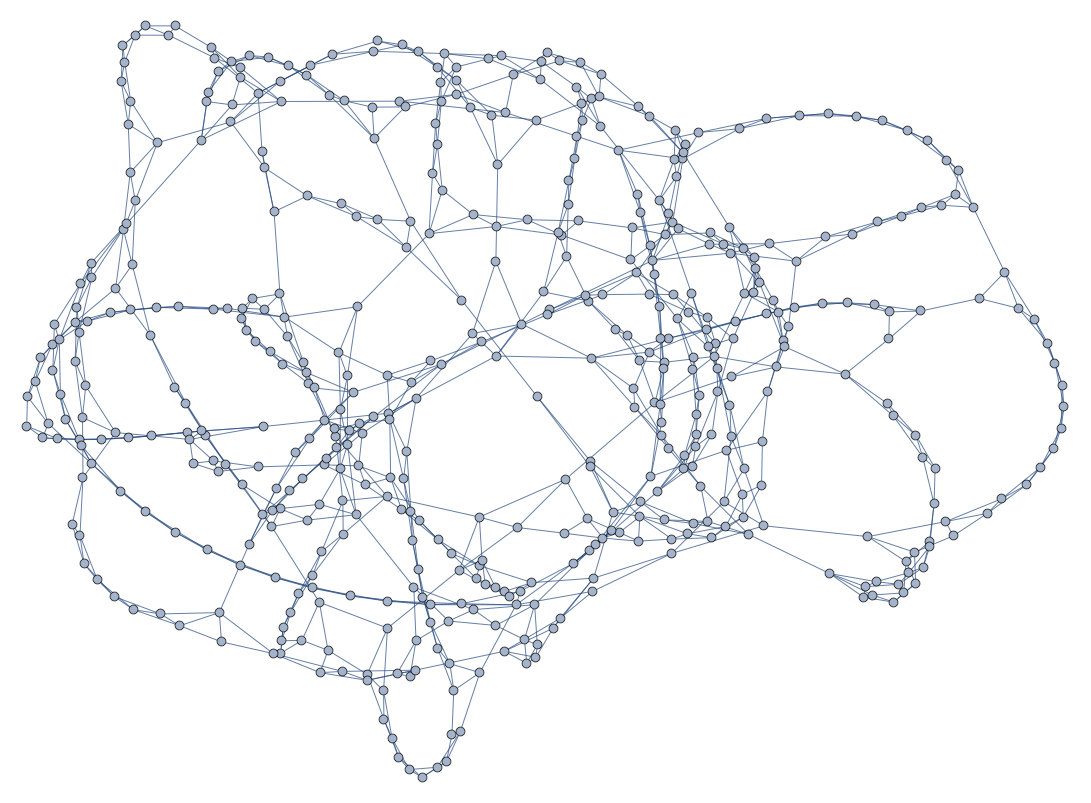
\includegraphics[width=1\linewidth]{watts-strogatz/500,0`5.png}
	\caption{A graph of 500 nodes created from the Watts-Strogatz model with a rewiring probability $0.5$}
	\label{fig:ba-700}
\end{figure}
\\
\\
The Watts-Strogatz model is constructed in two parts.
\begin{enumerate}[nosep]
	\item\label{w-s-1} \textit{Make a ring lattice} Take $n$ nodes. These are each given a number $i$. Then the $i^{\text{th}}$ node is connected to $K/2$ nodes below it and $K/2$ nodes above it, modulo $n$. 
	\item\label{w-s-2} \textit{Rewire} Then after this, for each pair of nodes, rewire them with probability $\beta$. To rewire an edge means to remove that edge and replace it with another that avoids loops or parallel edges.\\
\end{enumerate}
Step \ref{w-s-1} creates the high clustering and the random links introduced in step \ref{w-s-2} give the short average path lengths. The parameter $\beta$ mediates between these two characteristics. Indeed in the limit $\beta=1$, it approximates an Erd\H{o}s-R{\'e}nyi graph which as we've seen has low clustering. In the limit $\beta=0$ it is a ring lattice which has long average path lengths.\\
\\
However, it now fails where the Barab\'asi-Albert graphs succeeded in that its probability distribution is not as long-tailed as a real-network. Hence choosing between these two graphs is a trade-off. In practice the best choice depends on what features one is investigating.
%\subsubsection{Exponential Random Graphs}
%-- Wait for Data Science Institute talk on this next week --
\subsection{Real-world network datasets}
An alternative to using a random graph is to use a real-world dataset. For example, Facebook have access to a dataset of the social network of almost 2 billion people\cite{num-fb-users}. Whilst researcher's access to this data is becoming rapidly more limited due to very valid privacy concerns it is still easy to obtain a subset of this data by `scraping' the friends list of public profiles, as seen in Figure \ref{fig:facebook-network}. This has the problem that there are people who are not on Facebook and also that many users do not have their friend lists accessible to the public. A readily available and anonymised set of data can be found online\cite{fb-ego-data}. This is a graph of $4039$ nodes and $88234$ edges.\\
\\
Currently the largest open-source dataset of a social network is a dataset of the Friendster network\cite{friendster-data-archive}. This graph dwarfs the pre-organised Facebook data, containing $117,751,379$ nodes and $2,586,147,869$ directed edges. A slightly tamed version exists \cite{friendster-data-stanford} that takes the induced subgraph of users who are have at least some connection to the rest of the community, ignoring the stand-alone users. Whilst this is too large and unwieldy for this paper, a more manageable dataset could be attained by choosing a node and considering the induced graph of all nodes within a path of length, say, three from this node.\\
\\
For specific problems it may be worth conducting data gathering missions to map specific networks. For example sometimes research is done on specific communities such as the social networks of autistic school children\cite{anderson_locke_kretzmann_kasari_2015} or the relationships between Chilean astronomers\cite{chilean-astronomers}. The benefits of using datasets are that we know that the networks we are simulating on relate to some real-world network. This means we have some guarantee that it at least looks a bit like the underlying network we are trying to model.\\
\\
The negatives of this route are that it is just one instance of a network. It seems like, for example, the Facebook friendship network \textit{could} have looked differently but kept similar features. One way to deal with this shortcoming is by using exponential random graphs. This is a family of random graphs whose probability distribution is designed to make it highly likely that a graph drawn from this distribution shares certain key properties such as mean degree or degree distribution\cite{networks}. This feature has made them of use in modelling social networks\cite{exponential-random-graph}.
%\textit{Mark: I’d say something like “this is a family of random graphs whose probability distribution is designed to make it highly likely that a graph drawn from the distribution shares certain key properties—mean degree, or degree distribution—}
\label{mm}
%This is a family of random graphs that are generated in such a way that it makes it highly likely the a are graphs that can take the properties of the specific instance of the graph to created many more with the same properties\cite{networks}.
Another, less avoidable, problem is that network data that serves as a proxy or approximation for a real underlying data will often be incomplete, particularly if the dataset is large and automatically collected such as the Facebook or Friendster data.
\subsection{Example: Boltzmann wealth model on a network}
So far we have developed a model of the transfer of wealth that assumed that relationships between agents are homogeneous. That is, they can transfer money with every agent equally easily. We can think of the agents as nodes and the ability to transfer wealth between two agents as an edge. Then the model we were previously using is the equivalent of a complete graph, the graph in which each node is joined by an edge to every other\footnote{See Chapter \ref{ch:games-on-networks} for a primer on graph theory.}.\\
\\
As explored in the previous section, many real situations are not as homogeneous as this. Therefore it makes sense to consider cases in which some agents cannot transfer to others. To do this in an ABM we keep the agents the same but change the environment in which they exist and the rules they interact by.
\subsubsection{On a 2D Lattice}
One interesting thing to do is to make the environment a 2-dimensional lattice which the agents can move on. Then the nodes of the graph do not represent individual agents but spaces in which the agents can inhabit. That is we consider each agent as being at a certain position on a 2D lattice. We can add some rules to the Boltzmann wealth model to do this:
\begin{enumerate}[
%	label={Rule \arabic*}
	]
	\setcounter{enumi}{\value{rule}}
	\item At each tick, an agent moves to a neighbouring square.
	\item Multiple occupancy is allowed
	\item An agent can transfer money to any agent on a neighbouring square, including on their own square
\end{enumerate}
Implementing this requires that the individuals store two extra parameters: x and y position. They also need a method to allow them to both move position and check the position of other agents to see if they are neighbours.\\
\\
Implementing this on a 2D lattice with the Moore neighbourhood gives a new model with different dynamics. Running this program with 100 agents on a $10\times10$ grid and plotting the result after 100 ticks gives figure \ref{fig:space-1}. The graph shows the wealthiest agent in that square. Interestingly the wealthiest agents with $3$ or $4$ units of wealth are usually surrounded by a high proportion of agents with $0$ units of wealth.
\begin{figure}[!h]
	\centering
	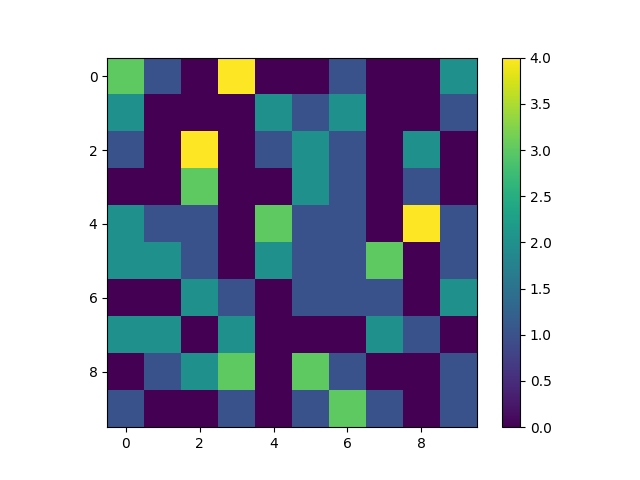
\includegraphics[width=.9\linewidth]{boltzmann-wealth/space-1.png}
	\caption{The Boltzmann wealth model on a 2D lattice. The grid on the left is the 2D lattice with the colours representing the wealth of the wealthiest agent in that square. Specifically yellow represents a wealth of $4$ and the dark blue a wealth of $0$.}
	\label{fig:space-1}
\end{figure}
\subsubsection{On an Barab\'asi-Albert network}
We can also consider the same basic model but on other types of network. Moving back to the assumption that  the agents are fixed in their neighbours and do not move, we let each agent be a node in the network. Running the simulation on a Barab\'asi-Albert network provides an interesting augmentation of the original model.\\
\\
We choose to perform 100 runs of this simulation with $50$ agents on an Barab\'asi-Albert network. Plotting the same graph of frequency density of wealth shows that the network simply amplifies the inequality we saw previously (Figure \ref{fig:network-ba-1}).
\begin{figure}[!h]
	\centering
	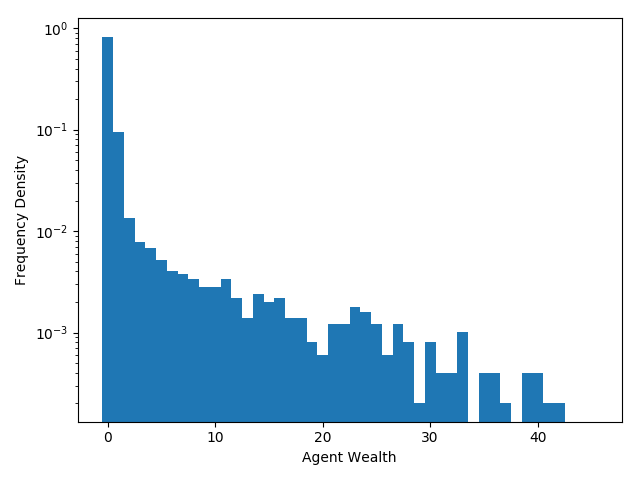
\includegraphics[width=.9\linewidth]{boltzmann-wealth/network-ba-1-log.png}
	\caption{Boltzmann wealth model on a Barab\'asi-Albert network. The resulting wealth inequality is so severe that the graph has to be plotted with a log scale on the y-axis. Around 80\% of the population have a wealth of $0$ while there are individuals with wealths of $40$.}
	\label{fig:network-ba-1}
\end{figure}
If we look in more detail we can see that the wealth of an agent is positively correlated to the degree of the node (Figure \ref{fig:network-ba-cor}). Now over $80\%$ of the population has $0$ units of wealth and some agents end runs with over $40$ units, constituting $80\%$ of the total wealth in their population.
\begin{figure}[h]
	\centering
	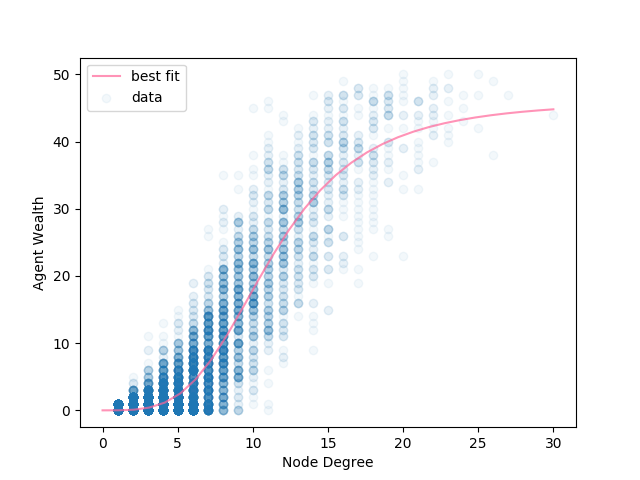
\includegraphics[width=.9\linewidth]{boltzmann-wealth/network-ba-cor2.png}
	\caption{Correlation between node degree and wealth in the Boltzmann wealth model on the Barab\'asi-Albert network. Each point represents the node degree of an agent and its wealth at the end of a run. This plot shows the result of 1000 runs each time running with 50 agents for 100 steps. The data is fit with a sigmoidal curve of best fit.}
	\label{fig:network-ba-cor}
\end{figure}

%Could say something about measures of gini
%To summarise, changing the underlying network of a model can have a major effect on the dynamics.
\section{Converting deterministic epidemiological models to ABMs}
We have learnt how ABMs can work, typical ways of analysing them and how the underlying network can affect the dynamics. With this we can move back towards studying epidemiology and revolutions. The first step we can make is to adapt the ideas from the deterministic compartmental models in Chapter \ref{ch:compartments} to an agent-based model on a network that can incorporate discreteness and stochasticity.
\subsection{Stochastic SIR model}
\subsubsection{Building the model}
%put on graph
We will start by adapting the simplest SIR compartmental model to make an ABM. The first step is to make the agents discrete. To do this we represent each agent as a node, creating $n$ nodes. We then have some edges joining them. We don't need to define the edges yet but we know that in general they join some nodes and not others. These edges together with the nodes form a graph $G$.\\
\\
%states and moving between states: infective to removed
The next step is to adapt the properties of classes in the population to properties of each agent. For example, instead of a class's size decreasing by a certain rate, we want each individual in that state to have a certain probability of moving to another state in any time. Previously we had three classes. To adopt this we have three states agents can be in: susceptible, infected and removed. Before we had that the infective class decreases at a rate of of $\alpha I$ whilst the infective class increases at the same rate. To adopt this we have that each individual moves from infective to removed with rate $\alpha$.\\
\\
%moving between states: susceptible to infective
Reinterpreting the movement from susceptible to infected takes a bit more thought. Previously to define the rate of contacts we assumed the law of mass action. However as we will incorporate a network structure for the environment, we are looking for something more sophisticated than this. Specifically we want to represent that some agents are more likely to come into contact than others.\\
\\
To do this it helps to break down the meaning of the contact rate $\beta$ from chapter \ref{ch:compartments}. Technically $\beta$ is the product of two parameters: the probability of contact between two individuals, $p$, and the probability of a contact leading to infection, $c$. In the previous compartmental model through the assumption of mass action we assumed that the probability of contact between any two individuals, $p$, was equal. However on a general network this is not true.\\
\\
Now we have $p=0$ for any non-neighbours and $p\neq0$ for neighbours. It makes intuitive sense for $c$ to be constant for any disease regardless of the model we are using. Therefore to make the values of $\beta$ we use comparable between the compartmental and agent-based models we need to adjust the value of $p$. Define $\hat n$ to be the average number of neighbours a node has. Let $\hat p$ be the probability of contact between two individuals in the network model. Then we need $\hat n \hat p = p N$. This ends up making the contact rate in the ABM $\hat\beta=\beta N/\hat n$.\\
%\\
%\textit{Mark: I see what you mean about this section. Do you have a clearer idea of what you want to say now?}
\label{mmd}
\\
Finally, mirroring the initial conditions we set just a single node as infective.\\
\\
We can summarise all of this succinctly:
\begin{enumerate}[nosep]
	\item There is a graph of $n$ nodes where each node is an individual
	\item The individual can be in one of three states: susceptible, infective or removed
	\item Two neighbouring individuals come into contact at a rate $p$. This contact rate is independent of the degrees of the two nodes.
%	\textit{Mark: Is this contact rate independent of the degrees (or number of neighbours) of the  two nodes?}
	\label{mmd}
	\item An infective infects a susceptible upon contact with probability $c$, after which the susceptible becomes infective
	\item Infectives are removed at a rate $\alpha$
	\item Initially there is a single node that is infective	
\end{enumerate}
\subsubsection{Running the simulation}
To support the agent-based modelling, the code uses the MESA framework. This is an open-source modular framework that aims to aid research in modelling, analysing and visualising agent-based systems in Python\cite{mesa-github}. Using MESA we can create an interactive sandpit for experimenting with different parameter values on this model (Figure \ref{fig:SIR-interactive}).
\begin{figure}[h]
	\centering
	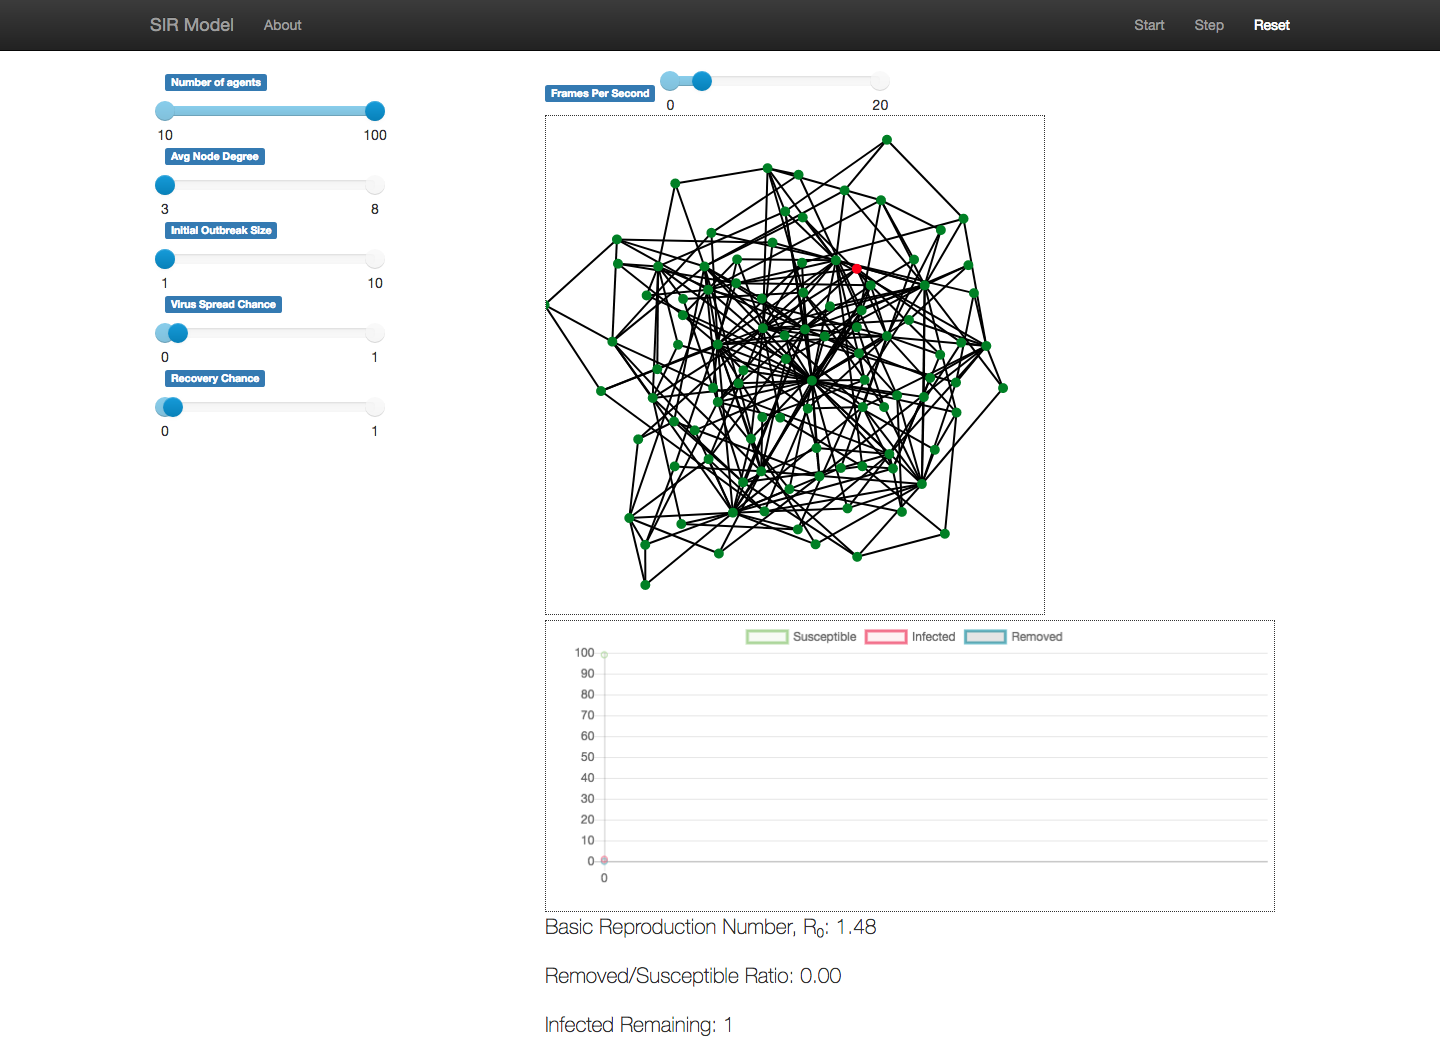
\includegraphics[width=\linewidth]{SIR-network/SIR-interactive.png}
	\caption{The interactive screen of the SIR model. We have a similar screen for all following ABMs. On the left we can adjust parameter values, in the centre there is a live view of the dynamic network, below that an updating graph of class size against time and at the bottom we have some key statistics such as the value of $R_0$. The top bar allows the user to stop and start the simulation as well as find out further information about the model.}
	\label{fig:SIR-interactive}
\end{figure}
\begin{figure}
	\centering
	\begin{subfigure}{.3\textwidth}
		\centering
		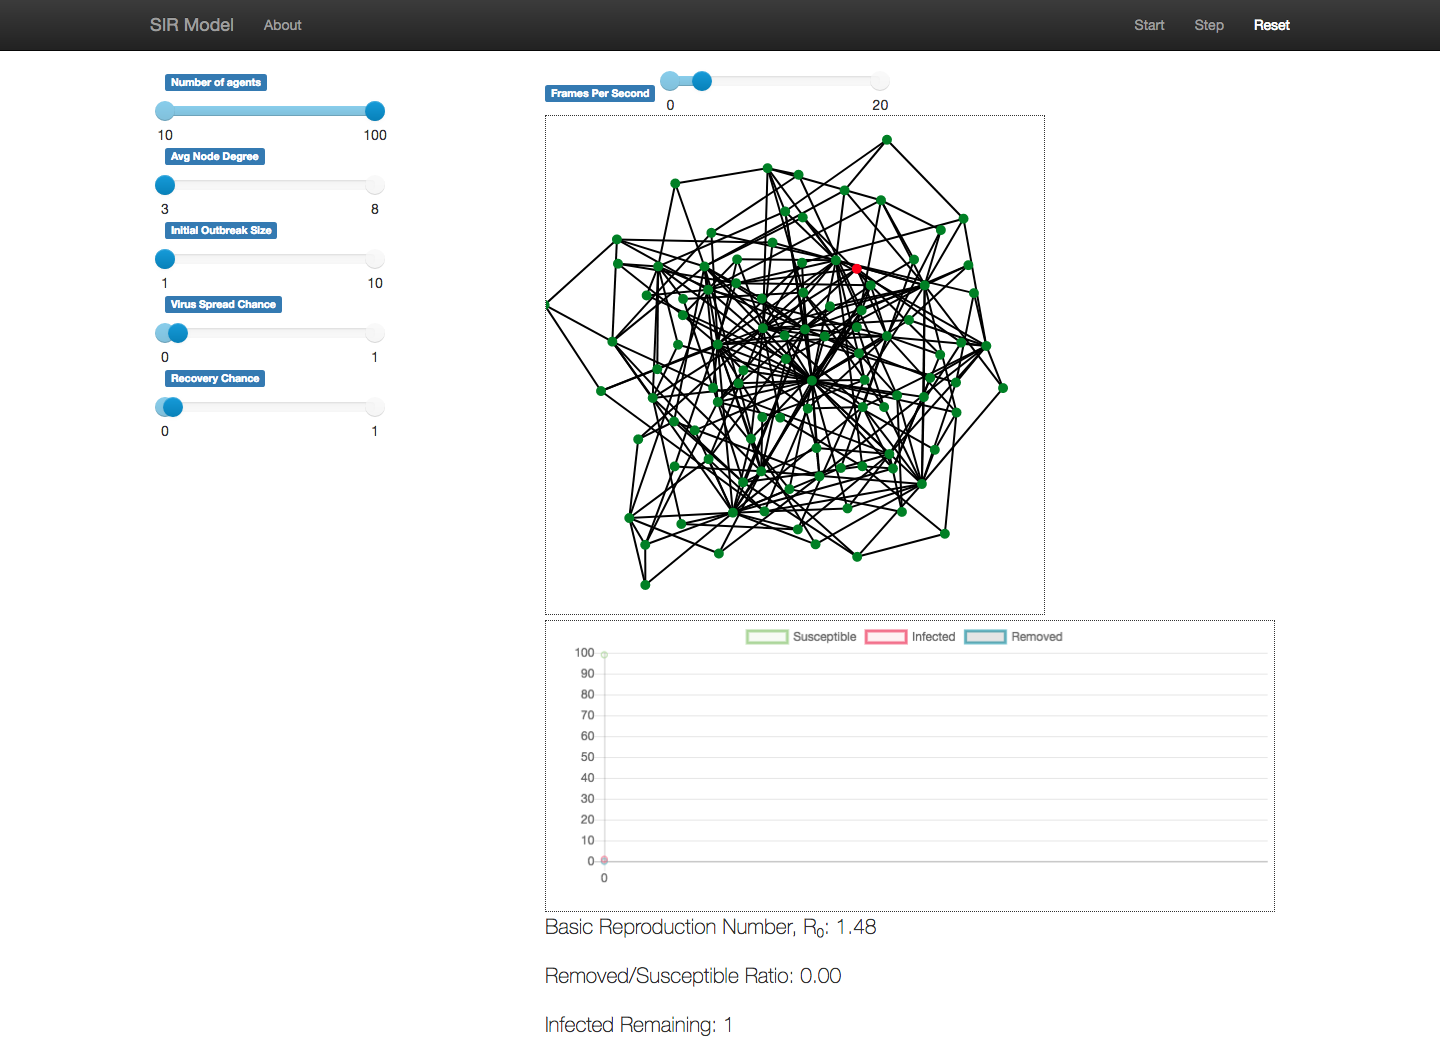
\includegraphics[width=1\linewidth,trim={19.275cm 16cm 14cm 4.5cm},clip]{SIR-network/SIR-interactive.png}
		\caption{$t=0$}
		\label{fig:SIR-network-1}
	\end{subfigure}%
\begin{subfigure}{.3\textwidth}
	\centering
	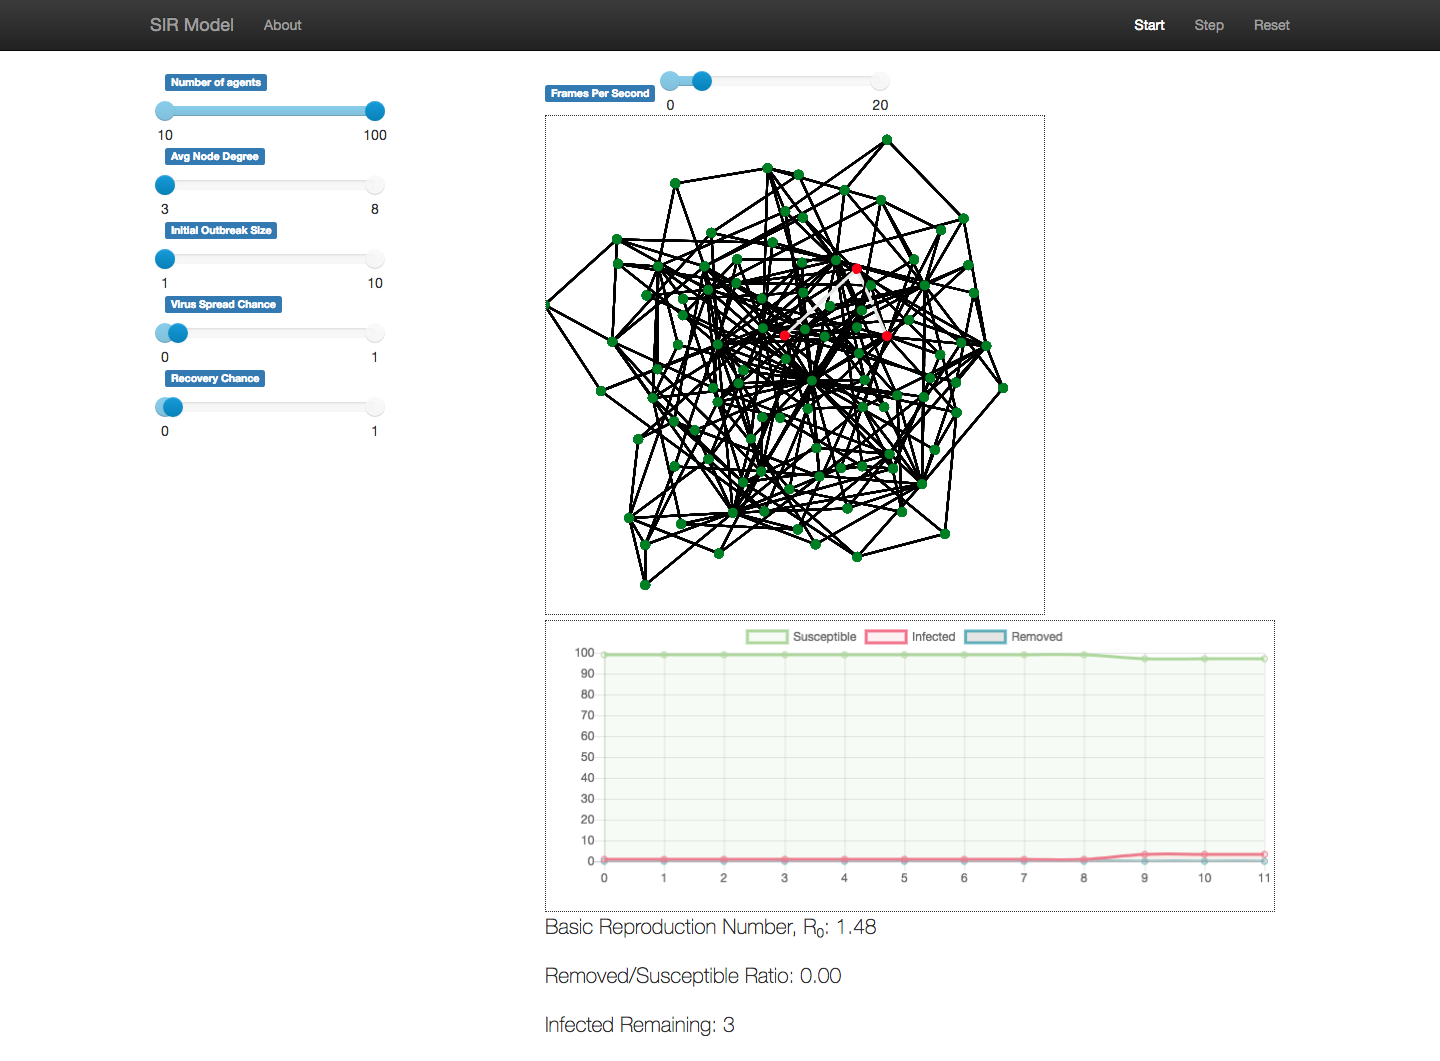
\includegraphics[width=1\linewidth,trim={19.275cm 16cm 14cm 4.5cm},clip]{SIR-network/SIR-interactive-2.png}
	\caption{$t=15$}
	\label{fig:SIR-network-2}
\end{subfigure}%
	\begin{subfigure}{.3\textwidth}
		\centering
		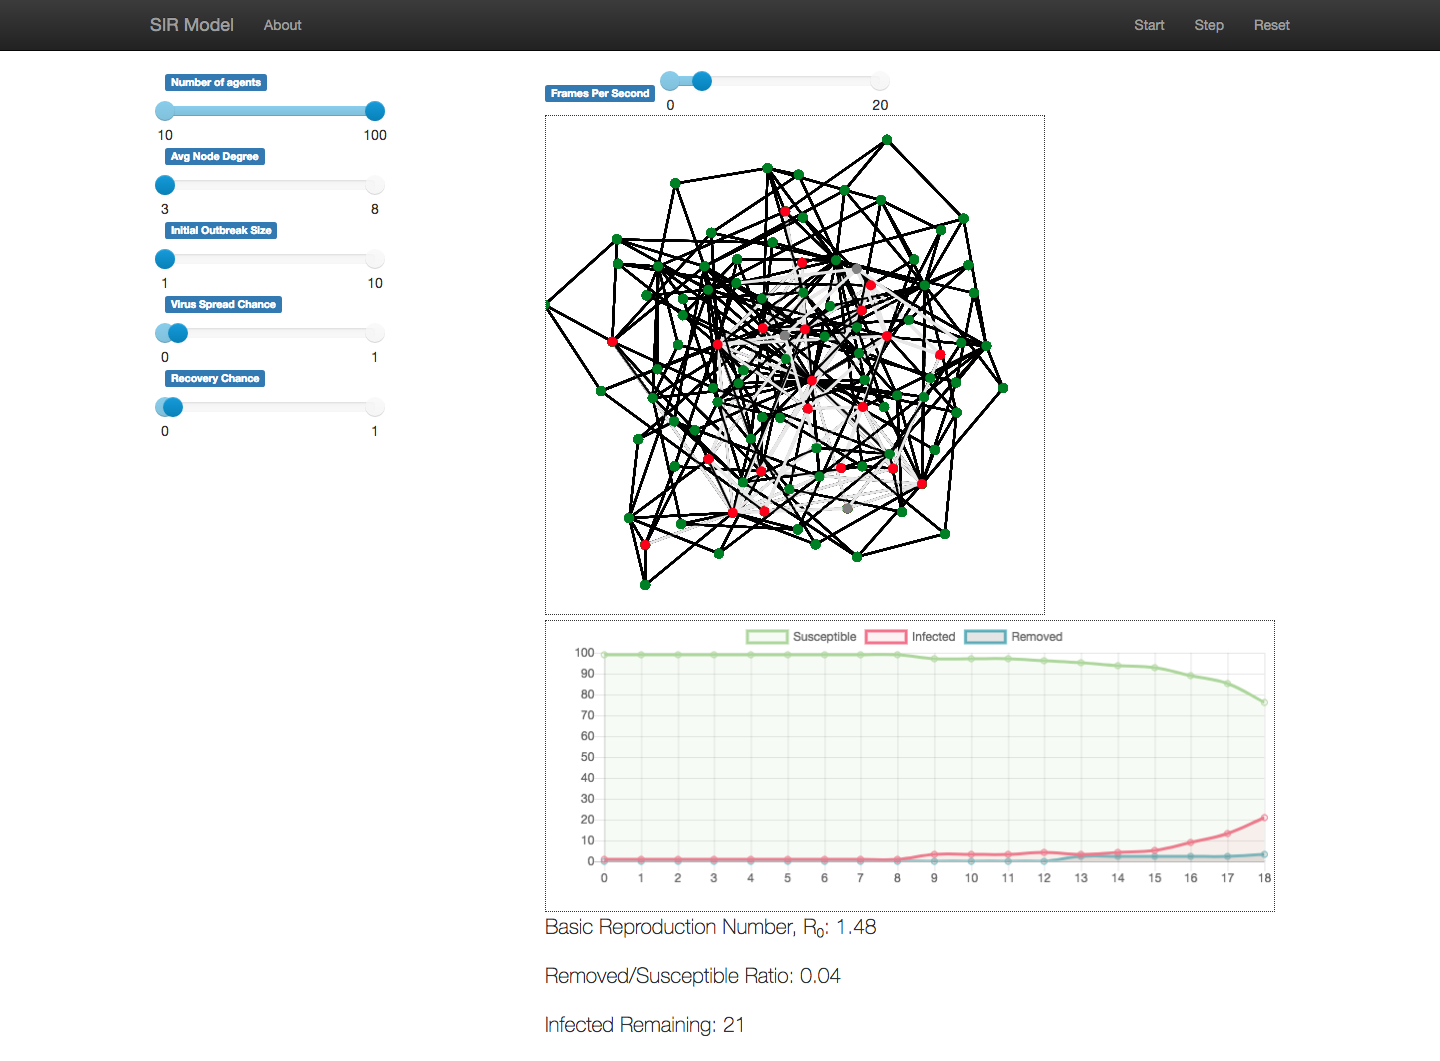
\includegraphics[width=1\linewidth,trim={19.275cm 16cm 14cm 4.5cm},clip]{SIR-network/SIR-interactive-3.png}
		\caption{$t=30$}
		\label{fig:SIR-network-3}
	\end{subfigure}
	\caption{The evolving network in the agent-based SIR model with $70$ nodes. Green, red and grey dots represent susceptible, infective and removed individuals respectively. Black edges represent that the infection could still be passed through that edge whilst grey edges mean that neither of the two nodes are susceptible.}
	\label{fig:SIR-network-run}
\end{figure}
\\
\\
We start by running a simulation with a small number of individuals (Figure \ref{fig:SIR-network-run}). We can see that this new model can reflect the fact that the growth of classes is stochastic, going both up and down, such as at the peak of the infective class's size in Figure \ref{fig:SIR-graph-1}.
\begin{figure}[h!]
	\centering
	\includegraphics[width=\linewidth]{SIR-network/1.png}
	\caption{A graph of the change in the three classes size through time in the agent-based SIR model with $70$ nodes.}
	\label{fig:SIR-graph-1}
\end{figure}\\
\\
With a higher number of individuals, if the revolution gets going we see that it is very smooth due to the law of large numbers (Figure \ref{fig:SIR-graph-2}). In this case we can see that the dynamics approximate the dynamics seen in the continuous compartmental models which is reassuring.
\begin{figure}[h!]
	\centering
	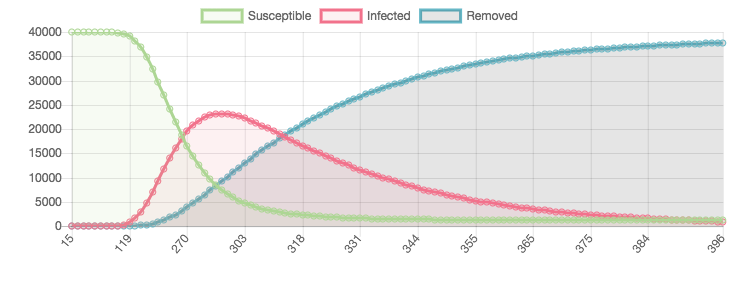
\includegraphics[width=\linewidth]{SIR-network/2.png}
	\caption{The SIR ABM with $40000$ agents.}
	\label{fig:SIR-graph-2}
\end{figure}\\
\\
The important distinction between the compartmental model and the ABM is that now the infection can die out even with $R_0>1$.
\begin{figure}[h!]
	\centering
	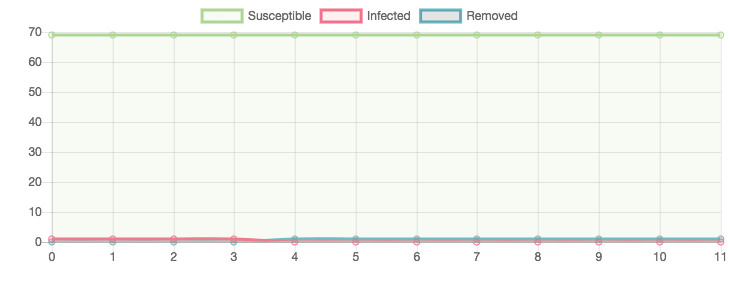
\includegraphics[width=\linewidth]{SIR-network/3.png}
	\caption{An infection dying out on the SIR model even with $R_0=1.07>1$}
	\label{fig:SIR-graph-3}
\end{figure}
The probability that the infection dies with the first infective is $\beta\hat n/(\alpha+\beta\hat n)$. This is because the time it takes on average for an infective to infect a susceptible is exponentially distributed with parameter $\beta \hat n$ where $\hat n$ is the average number of neighbours a node has. Also the time it takes for an infective to be removed is exponentially distributed with parameter $\alpha$. So the probability that the infection will run out in the early stages is $>\beta\hat n/(\alpha+\beta\hat n)$.
\subsection{Stochastic SEIR model}
Next, as before, we introduce the exposed class. Exposed nodes become active at a rate of $\gamma$ and active nodes are removed at a rate of $\alpha$. The mechanism for moving from susceptible to active now describes the move from susceptible to exposed. Again putting all of the rules in a list and using italics to highlight the rules that differ from the SIR model:
\begin{enumerate}[nosep]
	\item There is a graph of $n$ nodes where each node is an individual
	\item The individual can be in one of \textit{four} states: susceptible, \textit{exposed}, infective or removed
	\item Two neighbouring individuals come into contact at a rate $p$
	\item An infective infects a susceptible upon contact with probability $c$, after which the susceptible becomes \textit{exposed}
	\item \textit{Exposed individuals become infective at a rate $\gamma$}
	\item Infectives are removed at a rate $\alpha$
	\item Initially there is a single node that is infective
\end{enumerate}
\bigskip
Running this we see, as in the compartmental SEIR model that the introduction of the exposed class dampens the rate of increase in the infected population (Figure \ref{fig:SEIR-network-1}).
\begin{figure}[h!]
	\centering
	\includegraphics[width=\linewidth]{SEIR-network/1.png}
	\caption{}
	\label{fig:SEIR-network-1}
\end{figure}
Also because of the stochastic elements the model permits wipe-out even with $R_0>1$.
\subsection{Stochastic agent-based revolution model}\label{sec:abm-rev}
Now we can fully describe and implement a stochastic agent-based model of a revolution on a network.\\
\\
The movements from $S\rightarrow E$, $I\rightarrow R$ are the same as described in the SEIR model. However we need to incorporate a version of the non-linear movement from $E\rightarrow I$ that we devised in section \ref{sssec:zealots}. The part we need to adapt is the threshold $k$ for social influence. In the compartmental model of revolution $k$ was a fraction of the population which represented the threshold for non-zealots to become involved in a revolution. However, one of the key benefits of simulating on a network is that we do not assume each individual has an omniscient view of the population. Instead their view is highly localised and limited to their neighbours on the graph. So instead of a proportion of the population we want $k$ to represent a threshold for how many neighbours need to be active for an individual to become active. That is, the value given will be the number of active neighbours, $\hat i$, an exposed individual has to have for them to turn their idea into action. Based on the research we justified our previous decision with, this is around $3$ people\cite{asch-conformity}. So we now set $\hat k=3$. Then an exposed individual moves to active with probability
\begin{equation}\label{eq:non-zealot-abm}
\gamma \frac{\hat i^n}{k^n+\hat i^n}
\end{equation}
Further we give every agent an attribute: zealot or non-zealot. This determines if they will move to the active state when exposed with rate given by equation \ref{eq:non-zealot-abm} or the zealot rate $\delta$. This is a property held all the time by all agents and does not change. However it only affects their transition rate $E\rightarrow I$.\\
\\
Written out these rules are:
\begin{enumerate}[nosep]
	\item There is a graph of $n$ nodes where each node is an individual
	\item The individual can be in one of four states: susceptible, exposed, infective or removed
	\item \textit{Each individual is of one of two types: zealot or non-zealot}
	\item Two neighbouring individuals come into contact at a rate $p$
	\item An infective infects a susceptible upon contact with probability $c$, after which the susceptible becomes exposed
	\item \textit{If an exposed individual is a zealot, they become infective at a rate $\gamma \frac{\hat i}{k^n+\hat i^n}$}
	\item \textit{Otherwise if an exposed individual is a non-zealot they become infective at a rate $\delta$}
	\item Infectives are removed at a rate $\alpha$
	\item Initially there is a single node that is infective
\end{enumerate}
\bigskip
We choose to first run this model on a Watts-Strogatz network with 70 nodes (\ref{fig:abm-rev-70}). 
\begin{figure}[h]
	\centering
	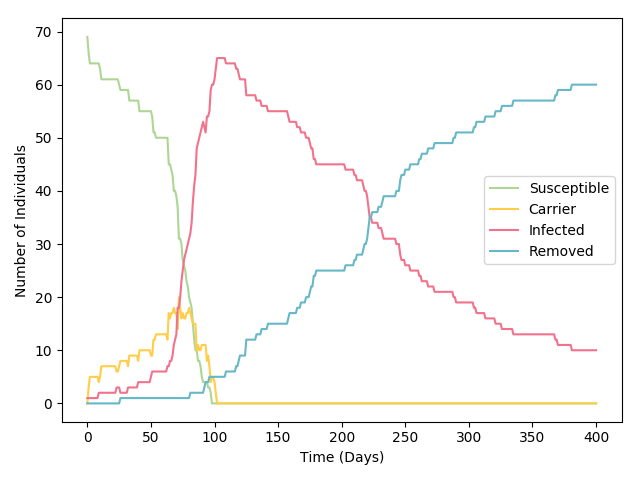
\includegraphics[width=\linewidth]{rev-abm/rev-ws.png}
	\caption{A typical trajectory using default parameters on a Watts-Strogatz network with $70$ agents.}
	\label{fig:abm-rev-70}
\end{figure}
Making the number of nodes much larger confirms that the model shares many qualitative properties with the previous compartmental model of Section \ref{sec:rev-compartment}.
\begin{figure}[h]
	\centering
	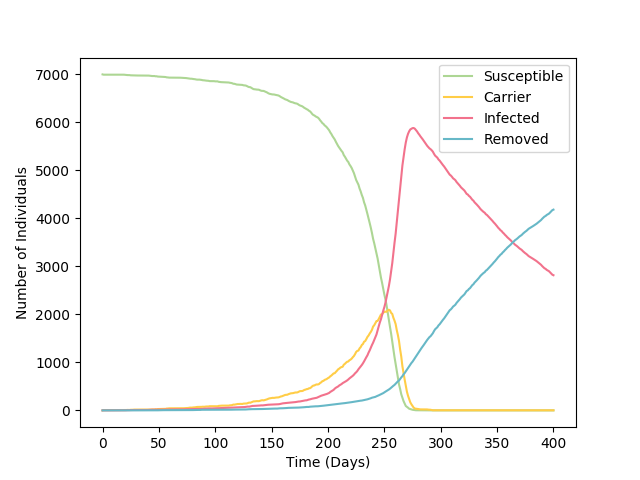
\includegraphics[width=\linewidth]{rev-abm/rev-abm-2.png}
	\caption{A typical trajectory using default parameters on a Watts-Strogatz network with $7000$ agents}
	\label{fig:abm-rev-7000}
\end{figure}
Again, importantly the model allows the possibility of the growth of the infective class ending prematurely even with $R_0>1$ meaning it does not follow the same qualitative pattern as the compartmental model. Whilst this is an obvious strength, there are many more benefits to this network model. However they are more nuanced and we need to interrogate the results from a network perspective to see them.
\subsubsection{The effects of an agent's limited perspective}
As we have moved from a homogeneous model to one which incorporates the limited perspective of individuals it is interesting to see how this creates localised dynamics. One interesting feature in this model is how the infectives and exposed classes are distributed within the network quite differently. The infectives are highly clustered, huddled around the original infective. However, the exposed class tends to be spread throughout the network.\\
\\
Intuitively, the infectives need the support of their community to be active. However, the long range links provided by the small world model mean that contacts occur between the infective population and outside communities. So occasionally the idea jumps out of the active population to further away communities who are not currently active. However, the receiver of this idea has no other actives in sight and so does little about it. This means they stay as exposed and do not transfer to active.
%\textit{Mark: stick to one term: exposed or active}
\label{mmd}
Instead they lie waiting for the action to reach them.\\
\\
To comment on this quantitatively we need some measure of clustering and spread of classes on networks. We do not want the measures to be explicitly dependent on the size of the class. We also choose to normalise the measure so that it is between $0$ and $1$ to help us compare between classes easily.\\
\\
One way to define clustering of classes is as the average fraction of neighbours of the same class a node in that class has. Formally, let $G$ be a graph of $n$ nodes. Each node is in exactly one state $c_i$. In our model $c_i$ is equal to one of the states susceptible, exposed, infective or removed. Let the class $C_i$ be the set of all nodes in state $c_i$. Then $\abs{C_i}$ corresponds to the size of one of the compartments $S,E,I,R$ as given in the compartmental models. Write the neighbourhood of vertex $v$, excluding vertex $v$, as $N(v)$. We write $v\in C_i$ if $v$ is in state $c_i$.
%\textit{Mark: where the state of the $i$-th node is $c_i$. Joe: I don't mean that but clearly the notation is not very clear}
\label{mmd}
Then the clustering of class $C_i$ is
\[\Gamma_i(t)=\frac{1}{\abs{C_i}}\sum_{v\in C_i}\frac{\abs{N(v)\cap C_i}}{\abs{N(v)}}\]
\\
\\
To define spread, the idea that we want to capture is that the exposed class is more homogeneously spread through the network. One desirable option would be to calculate the shortest path from each node that is not in a state $c_i$ to a node in state $c_i$. However, calculating shortest paths is computationally very expensive. Instead we can approximate this by seeing if the shortest path is of length $1$. That is to say we see if the node has a neighbour in state $c_i$.\\
\\
We define spread of type as the proportion of number of nodes not in state $c_i$ that have a neighbour in state $c_i$. Let $\theta_i$ be a characteristic function indicating if a set of nodes has a node of type $c_i$
\[\theta_i(X)= \left\{\begin{array}{lr}
1, & \text{if } X\cap C_i\neq\emptyset\\
0, & \text{otherwise}
\end{array}\right\}\]
Then
\[S_i(t)=\frac{1}{n-\abs{C_i}}\sum_{v\in V(G)\setminus C_i} \theta_i(N(v)) \]
\\
\\
With these two measures we can test the clustering and diffusion quantitatively. Running a simulation we find that the two populations do indeed cluster and spread as described (Figure \ref{fig:clustering-diffusion-rev-abm}). The idea spreads through the population widely, even when the revolution is not very developed, as seen from Figure \ref{fig:diffusion-rev-abm}. The community of revolutionaries tends to be very clustered (Figure \ref{fig:clustering-rev-abm}). However, the community of people who have the idea is unclustered and spread out. This provides suitable foundations for when the revolution does actually arrive. As we can see the exposed class is quickly depleted as more people become active.
\begin{figure}
	\centering
	\begin{subfigure}{\textwidth}
		\centering
		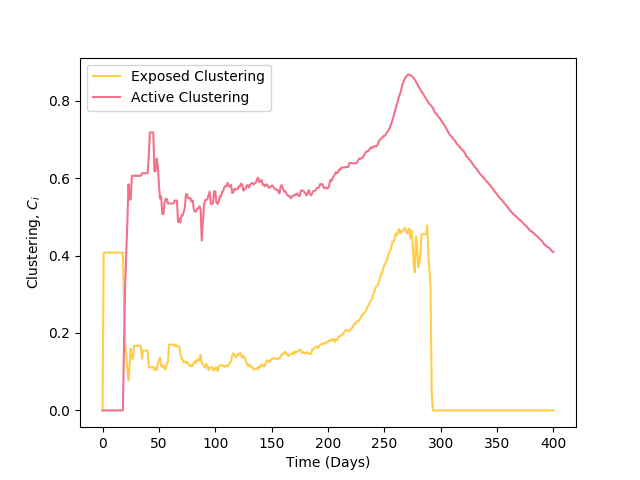
\includegraphics[width=0.9\linewidth]{rev-abm/clustering2.png}
		\caption{Clustering}
		\label{fig:clustering-rev-abm}
	\end{subfigure}%
\\
	\begin{subfigure}{\textwidth}
		\centering
		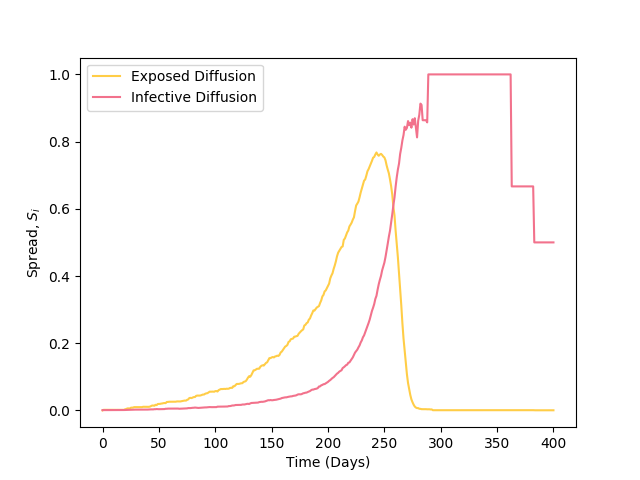
\includegraphics[width=0.9\linewidth]{rev-abm/diffusion2.png}
		\caption{}
		\label{fig:diffusion-rev-abm}
	\end{subfigure}
	\caption{Clustering and spread in the revolution ABM with default parameters. Figure \ref{fig:clustering-rev-abm} shows that the active population is consistently more clustered than the exposed population. Figure \ref{fig:diffusion-rev-abm} shows that the exposed class increase their spread through the population before being suddenly depleted near the peak of the revolution as they convert to the rapidly burgeoning active population.\label{mmd}}
	\label{fig:clustering-diffusion-rev-abm}
\end{figure}
\\
\begin{tcolorbox}
	\paragraph{Lesson for revolutionaries:} Ideas travel further than action. The idea can be widely distributed and lie dormant until action reaches it.
\end{tcolorbox}
\section{The Empire Strikes Back}
An interesting option is to introduce an adversarial agent to the model: the regime. It is an interesting question to ask what tactics they should adopt. In the previous model we have an equal chance of each active individual being removed. Instead we allow the option of the regime removing nodes based on their properties.\\
%\\
%To distinguish this from the current case, it would be most revealing to simulate on an Barab\'asi-Albert graph as this has a probability distribution closer to real world networks and will provide more insight into a principle that relies on the distribution of node degree.\\
\\
To stop the revolutionary idea spreading the regime wants to limit the number of nodes the idea can reach. The most effective way to do this is to separate the graph into two components with one containing all active revolutionaries and the other containing the rest. This means the regime could use Menger's Theorem to disconnect the graph efficiently.
%\textit{Mark: tell us what Menger's theorem is}
\label{mmd}
Menger's Theorem states that the minimum number of nodes one needs to remove to disconnect two disjoint subgraphs $U, V\subset V(G)$ is equal to $k$, the number of distinct paths from $U$ to $V$\cite{graph-theory-reference}. In our example $U$ can be the set of exposed and infective nodes and $V$ the set of susceptible and removed nodes. These are clearly disjoint as a node is in exactly one of these states at one time so Menger's theorem for these two sets. The regime could then instantaneously remove $k$ active nodes to disconnect the two subgraphs. 
However, the assumption that the regime is able to identify and efficiently take out just the nodes that will separate the graph is incredibly strong, requiring exact knowledge of the network and the ability to pick out any individual.\\
\\
Instead we assume that the regime becomes aware of revolutionaries only through attempted contacts with susceptibles. With this ability, what is the best option for the regime? It makes sense for them to pick out active revolutionaries with the highest number of contacts. This makes the problem one of attack tolerance in networks\cite{attack-tolerence-network}. In practice this means that more high-profile revolutionaries are at greater risk. This is based on the idea everyone is at some risk and this is proportional to the number of contacts $p\hat n$ they can and do make. Based on historical evidence this is often what happens: regimes target high-profile individuals both because they are more easily detected as well as them making a better example. Whilst this can provoke the populace it can also serve to provide a split in tactics and leadership. For these reasons we will consider this option.\\
\\
Some graphs are more resilient to this targeted node removal than others. Scale-free graphs have a low attack tolerance as removing just a few supernodes can drastically disconnect the graph. However, in a more egalitarian network such as the Watts-Strogatz network or Erd{\H{o}}s-R{\'{e}}nyi graph this is harder to do\cite{attack-tolerence-network}.\\
\\
Some naturally occurring networks seem to be naturally catered to tolerating attacks and failures. The social network of the bottlenose dolphins community of Doubtful Sound fjord has been studied in detail and shows an unusually high level of interconnection with no clear hubs and also low clustering\cite{dolphin-network}. The network was found by taking observations of a community of 64 dolphins over 6 years. There is an edge between two dolphins if they are seen together more often than expected by chance.
\label{mmd} The result of this network organisation is that if a few dolphins die it is very unlikely to break apart the social network and so they will stay as a single component. That is, they have evolved to have a high failure tolerance.\\
\\
The findings of the benefits of decentralised movements reflects a growing historical trend of egalitarian organisation in successful non-violent resistance\cite{battle-of-seattle}. As Eddie Yuen writes in \textit{The Battle of Seattle} on the trends that developed through the 20th century to lead to the increasing success of non-violent protest\cite{logic-non-violence} and in particular the Seattle protests against the WTO in 1999:
\begin{quote}
	The second [of these adoptions] is a commitment to direct democracy, as specifically the organisational forms of the affinity group, decentralized spokes-council meetings and consensus process.
\end{quote}
\begin{tcolorbox}
	\paragraph{Lesson for revolutionaries:} \textit{Be like a dolphin}. Decentralised and interwoven networks are more immune to targeted attacks. Pursue organisational structures which avoid unnecessary hierarchy by pursuing tactics such as direct democracy.
\end{tcolorbox}
%\section{Revolution on a Network}
%\subsection{Model Specification}
%This model involves one category of actors: 'citizens'. Following Epstein\cite{epstein}, we include two exogenous factors: hardship ($H$) and legitimacy ($L$).\\
%$H$ 
%\subsection{Agent Specification}
%They are members of the general population and may be in one of four states: susceptible ($S$), inactive revolutionaries ($I_1$), active revolutionaries ($I_2$), and removed ($R$). As in many agent-based models, they are heterogeneous in many respects.
